\newpage
\section{Auswertung}
\label{sec:Auswertung}
\subsection{Photodiode}
Zu 5.)\\

\begin{figure}
    \centering
    \includegraphics[width=0.5\textwidth]{build/plotLED.pdf}
    \caption{Messwerte - Spannung der Photodiode/Entfernung der LED}        
    \label{fig:plotLED}
\end{figure}

\begin{figure}
    \centering
    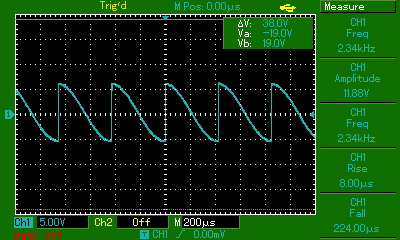
\includegraphics[width=0.5\textwidth]{bilder/MAP001.png}
    \caption{Phase 0° ohne Rauschen}        
    \label{fig:MAP001}
\end{figure}

\begin{figure}
    \centering
    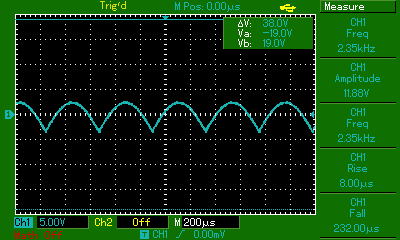
\includegraphics[width=0.5\textwidth]{bilder/MAP002.png}
    \caption{Phase 90° ohne Rauschen}        
    \label{fig:MAP002}
\end{figure}

\begin{figure}
    \centering
    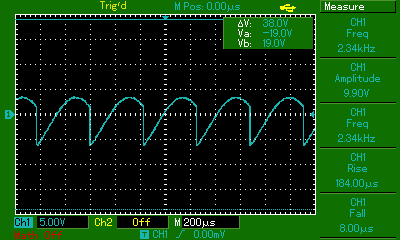
\includegraphics[width=0.5\textwidth]{bilder/MAP005.png}
    \caption{Phase 135° ohne Rauschen}        
    \label{fig:MAP005}
\end{figure}

\begin{figure}
    \centering
    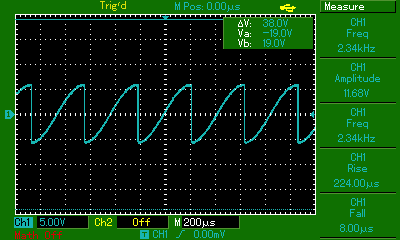
\includegraphics[width=0.5\textwidth]{bilder/MAP003.png}
    \caption{Phase 180° ohne Rauschen}        
    \label{fig:MAP003}
\end{figure}

\begin{figure}
    \centering
    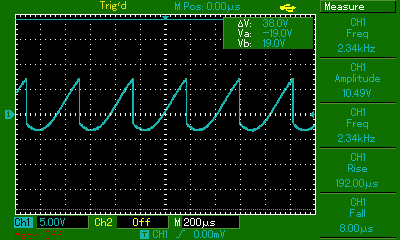
\includegraphics[width=0.5\textwidth]{bilder/MAP004.png}
    \caption{Phase 225° ohne Rauschen}        
    \label{fig:MAP004}
\end{figure}

\begin{figure}
    \centering
    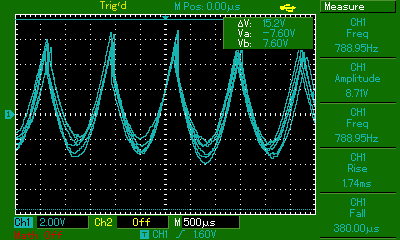
\includegraphics[width=0.5\textwidth]{bilder/MAP007.png}
    \caption{Phase 0° mit Rauschen}        
    \label{fig:MAP007}
\end{figure}

% \begin{figure}
%     \centering
%     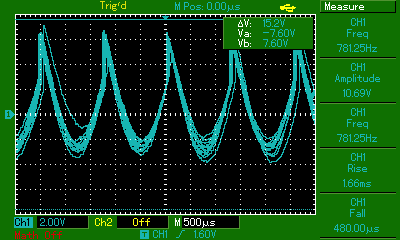
\includegraphics[width=0.5\textwidth]{bilder/MAP008.png}
%     \caption{MAP008}        
%     \label{fig:MAP008}
% \end{figure}

\begin{figure}
    \centering
    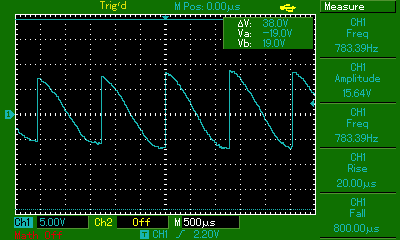
\includegraphics[width=0.5\textwidth]{bilder/MAP009.png}
    \caption{Phase 90° mit Rauschen}        
    \label{fig:MAP009}
\end{figure}

\begin{figure}
    \centering
    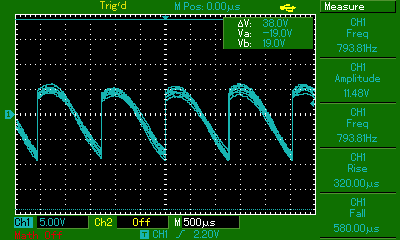
\includegraphics[width=0.5\textwidth]{bilder/MAP010.png}
    \caption{Phase 135° mit Rauschen}        
    \label{fig:MAP010}
\end{figure}

\begin{figure}
    \centering
    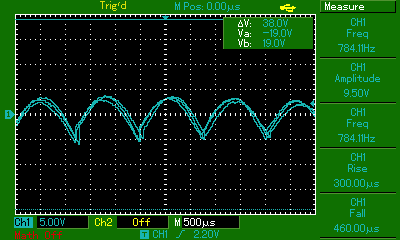
\includegraphics[width=0.5\textwidth]{bilder/MAP011.png}
    \caption{Phase 180° mit Rauschen}        
    \label{fig:MAP011}
\end{figure}

\begin{figure}
    \centering
    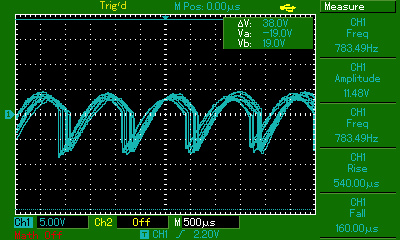
\includegraphics[width=0.5\textwidth]{bilder/MAP012.png}
    \caption{Phase 225° mit Rauschen}        
    \label{fig:MAP012}
\end{figure}
